\begin{dang}{Bài toán tìm m để hàm số đồng biến (nghịch biến) trên khoảng cho trước}
\begin{enumerate}[\iconCV]
\item Xét hàm số bậc ba $y=ax^3+bx^2+cx+d$ có $y'=3ax^2+2bx+c$.
	\begin{listEX}[1]
		\item [\ding{172}] Hàm số đồng biến trên  $\mathbb{R}$ khi và chỉ khi $$y' \ge 0,\,\forall x \in \mathbb{R} \Leftrightarrow \heva{&a>0\\&\Delta_{y'}\le 0}.$$
		\item [\ding{173}] Hàm số nghịch biến trên  $\mathbb{R}$ khi và chỉ khi $$y' \le 0, \,\forall x \in \mathbb{R} \Leftrightarrow \heva{&a<0\\&\Delta_{y'}\le 0}.$$
	\end{listEX}
\textit{Trường hợp hệ số $a$ có chứa tham số, ta kiểm tra thêm trường hợp $a=0$.}
\item Xét hàm phân thức $y=\displaystyle\frac{ax+b}{cx+d}$ có $y'=\dfrac{ad-cb}{(cx+d)^2}$, với $ad-cb \ne 0$ và $c \ne 0$.
\begin{itemize}
	\item [\ding{172}] Hàm số đồng biến trên từng khoảng xác định của nó khi và chỉ khi
	$$y'>0,\, \forall x \ne -\dfrac{d}{c}\Leftrightarrow ad-cb>0.$$
	\item [\ding{173}]  Hàm số nghịch biến trên từng khoảng xác định của nó khi và chỉ khi
	$$y'<0,\, \forall x \ne -\dfrac{d}{c}\Leftrightarrow ad-cb<0.$$
\end{itemize}
\item Xét hàm phân thức $y=\displaystyle\frac{ax^2+bx+c}{dx+e}$ có $y'=\dfrac{adx^2+2aex+be-dc}{(dx+e)^2}$, với $ad \ne 0$.
\begin{itemize}
	\item [\ding{172}] Hàm số đồng biến trên từng khoảng xác định của nó khi và chỉ khi
	$$y'\ge 0,\, \forall x \ne -\dfrac{e}{d}\Leftrightarrow adx^2+2aex+be-dc\ge 0,\, \forall x \ne -\dfrac{e}{d}.$$
	\item [\ding{173}]  Hàm số nghịch biến trên từng khoảng xác định của nó khi và chỉ khi
	$$y'\le 0,\, \forall x \ne -\dfrac{e}{d}\Leftrightarrow adx^2+2aex+be-dc\le 0,\, \forall x \ne -\dfrac{e}{d}.$$
\end{itemize}
\end{enumerate}
\end{dang}
\boxmini{BÀI TẬP TỰ LUẬN}
\setcounter{vd}{0}

\begin{vd}
	Tìm tất cả giá trị của tham số $m$ để hàm số
	\begin{tasks}
		\task $y=x^3+mx^2+2mx+2$ đồng biến trên $(-\infty;+\infty)$.
		\task $y=-\dfrac{1}{3}x^3-mx^2+\left(2m-3\right)x-m+2$ nghịch biến trên $\mathbb{R}$.
		\task $ y=\dfrac{1}{3}x^3-mx^2-(2m+1)x+1$ nghịch biến trên khoảng $(0;5)$.
		\task $y=x^3-3x^2+(5-m)x$ đồng biến trên khoảng $(2;+\infty)$.
	\end{tasks}
\loigiai{
\begin{enumerate}[a)]
	\item Hàm số đã cho có tập xác định $\mathscr{D}=\mathbb{R}$ và $y'=3x^2+2mx+2m$.\\
	Hàm số đã cho đồng biến trên $\mathbb{R}$ khi và chỉ khi
	\[y'\ge0,~\forall x\in\mathbb{R}\Leftrightarrow m^2-6m\le0\Leftrightarrow 0\le m\le6.\]
	\item Tập xác định: $D=\mathbb{R}$. Ta có $y'=-x^2-2mx+2m-3$.\\
	Để hàm số nghịch biến trên $\mathbb{R}$ thì:\\
	$y'\le 0,\forall x\in\mathbb{R} \Leftrightarrow\left\{
	\begin{aligned}
		&a_{y'}<0\\
		&\Delta'\le 0
	\end{aligned}
	\right.
	\Leftrightarrow \left\{
	\begin{aligned}
		&-1<0\\
		&m^2+2m-3\le0
	\end{aligned}
	\right.
	\Leftrightarrow -3\le m\le 1$.
	\item Tập xác định $\mathscr{D}=\mathbb{R}$.\\
	Ta có $y'=x^2-2mx-(2m+1)$, $ y'=0\Leftrightarrow\hoac{&x=-1\\&x=2m+1.}$\\
	Nếu $2m+1\leq-1\Leftrightarrow m\leq-1$ thì $y'\leq 0\Leftrightarrow x\in\left[2m+1;-1\right]$.\\
	Suy ra hàm số không nghịch biến trên khoảng $(0;5)$. \\
	$\Rightarrow m\leq-1$ không thỏa mãn.\\
	Nếu $2m+1>-1\Leftrightarrow m>-1$ thì $y'\leq 0\Leftrightarrow x\in\left[-1;2m+1\right]$.\\
	Để hàm số nghịch biến trên khoảng $(0;5)$ thì ta có $2m+1\geq 5\Leftrightarrow m\geq 2$.
	\item \textbf{\underline{Cách 1:}} Tập xác định $\mathscr{D}=\mathbb{R}$.\\
	Ta có $y'=3x^2-6x+5-m$.\\
	Hàm số $y=x^3-3x^2+(5-m)x$ đồng biến trên khoảng $(2;+\infty)$ khi và chỉ khi
	\allowdisplaybreaks
	\begin{eqnarray*}
		&&y'\ge 0,\,\forall x\in (2;+\infty)\\
		&\Leftrightarrow& 3x^2-6x+5-m\ge 0,\,\forall x\in (2;+\infty)\\
		&\Leftrightarrow& m\le 3x^2-6x+5, \,\forall x\in (2;+\infty)
	\end{eqnarray*}
	Xét hàm $g(x)=3x^2-6x+5$ trên $(2;+\infty)$ có $g'(x)=6x-6$ và $g'(x)=0\Leftrightarrow x=1$.\\
	Bảng biến thiên của $g(x)$
	\begin{center}
		\begin{tikzpicture}
			\tkzTabInit[nocadre=false,lgt=1.5,espcl=2,deltacl=0.5]
			{$x$/0.6,$g'(x)$/0.6,$g(x)$/1.5}
			{$2$,$+\infty$}
			\tkzTabLine{,+,}
			\tkzTabVar{-/$5$,+/$+\infty$}
		\end{tikzpicture}
	\end{center}
	Dựa vào bảng biến thiên của $g(x)$, ta được
	$$m\le 3x^2-6x+5, \,\forall x\in (2;+\infty) \Leftrightarrow m\le 5.$$
	\textbf{\underline{Cách 2:}} Tập xác định $\mathscr{D}=\mathbb{R}$.\\
	Ta có $y'=3x^2-6x+5-m$.\\
	Hàm số $y=x^3-3x^2+(5-m)x$ đồng biến trên khoảng $(2;+\infty)$ khi và chỉ khi
	$$y'\ge 0,\,\forall x\in (2;+\infty) 
	\Leftrightarrow \heva{& y'(2)\ge 0 \\ & -\dfrac{b}{2a} \le 2} 
	\Leftrightarrow \heva{& 5-m\ge 0 \\ & 1 \le 2}
	\Leftrightarrow m \le 5. $$
\end{enumerate}}
\end{vd}

\begin{vd}
	Tìm tất cả giá trị của tham số $m$ để hàm số
	\begin{tasks}
		\task $y=\dfrac{mx+2}{x+1}$ đồng biến trên từng khoảng xác định.
		\task $y=\dfrac{mx-2}{x+m-3}$ nghịch biến trên các khoảng xác định
		\task $y = \dfrac{mx-8}{x-2m}$ đồng biến trên $(3;+\infty )$.
		\task $y=\dfrac{mx+9}{4x+m}$ nghịch biến trên khoảng $(0;4)$.
	\end{tasks}
\loigiai{
\begin{enumerate}[a)]
	\item Từ yêu cầu bài toán, $\forall x \neq -1$ ta xét $y'>0$ $\Leftrightarrow m-2>0 \Leftrightarrow m>2$.
	\item Tập xác định $\mathbb{R}\setminus\{3-m\}$.\\
	$y' = \dfrac{m(m - 3) + 2}{\left( x + m - 3\right)^2} = \dfrac{m^2 - 3m + 2}{\left(x + m - 3\right)^2}$. \\
	Điều kiện để hàm số nghịch biến trên các khoảng xác định của nó là $y' < 0,\,\forall x \ne 3 - m$ hay $m^2 - 3m + 2 < 0 \Leftrightarrow m \in (1;2)$.
	\item Tập xác định: $\mathscr{D} = \mathbb{R} \setminus \{2m\}$.\\
	$y' = \dfrac{-2m^2+8}{(x-2m)^2}$.\\
	Hàm số luôn đơn điệu trên từng khoảng xác định $(-\infty; 2m)$ và $(2m; +\infty)$ khi $-2m^2 + 8 \ne 0$.\\
	Vậy hàm số đồng biến trên $(3;+\infty)$ khi và chỉ khi $-2m^2+8 > 0$ và $(3;+\infty) \subset (2m ;+\infty)$. \\
	Điều này tương đương $\heva{&-2<m<2\\&2m \le 3}$, hay $-2 < m \le \dfrac{3}{2}$.
	\item Tập xác định $\mathscr{D}=\mathbb{R}\setminus\left\{-\dfrac{m}{4}\right\}$.\\
	Ta có $y=\dfrac{mx+9}{4x+m}\Rightarrow y'=\dfrac{m^2-36}{(4x+m)^2}$.\\
	Để hàm số nghịch biến trên khoảng $(0;4)$ thì
	$$\heva{& y'<0 ,\forall x\in(0;4)\\ & -\dfrac{m}{4}\notin (0;4)}\Leftrightarrow\heva{& m^2-36<0 \\ &\hoac{&-\dfrac{m}{4}\geq4\\&-\dfrac{m}{4}\leq 0}}\Leftrightarrow\heva{& -6<m<6 \\ &\hoac{&m\leq-16\\&m\geq 0}}\Leftrightarrow 0\leq m<6.$$
\end{enumerate}}
\end{vd}

\begin{vd}
	Tìm tất cả giá trị của tham số $m$ để hàm số
	\begin{tasks}
		\task $ y = \dfrac{2x^2+3x+m+1}{x+1} $ đồng biến trên các khoảng xác định.
		\task $y=\dfrac{x^2+(m+1)x-1}{2-x}$ ($m$ là tham số) nghịch biến trên mỗi khoảng xác định.
	\end{tasks}
	\loigiai{
		\begin{enumerate}[a)]
			\item Tập xác định: $\mathbb{R}\setminus\{-1\}$.\\
			Ta có $y'=\dfrac{2x^2+4x+2-m}{(x+1)^2}$. Hàm số đồng biến trên các khoảng xác định khi 
			$$2x^2+4x+2-m\ge 0, \forall x\in \mathbb{R} \Leftrightarrow m\le \min\limits{\mathbb{R}\setminus \{-1\} } (2x^2+4x+2) = 0.$$
			\item Tập xác định $\mathscr{D}=\mathbb{R}\backslash\{2\}$.\\
			Đạo hàm: $y'=\dfrac{-x^2+4x+2m+1}{(2-x)^2}=\dfrac{g(x)}{(2-x)^2}$.\\
			Hàm số nghịch biến trên mỗi khoảng xác định của nó khi và chỉ khi $y'\le 0,\forall x\in \mathscr{D}$ (Dấu \lq\lq $=$\rq\rq~ chỉ xảy ra tại hữu hạn điểm thuộc $\mathscr{D}$).\\
			$\Leftrightarrow g(x)=-x^2+4x+2m+1\le 0,$  $\forall x\in \mathbb{R}$\\
			Điều kiện: ${\Delta}'\le 0$ (vì $a=-1<0$) $\Leftrightarrow 4-(-1)\cdot(2m+1)\le 0\Leftrightarrow 2m+5\le 0\Leftrightarrow m\le -\dfrac{5}{2}$.
	\end{enumerate}}
\end{vd}

\boxmini{BÀI TẬP TRẮC NGHIỆM}
\ind{PHẦN I.} \inden{Câu trắc nghiệm nhiều phương án lựa chọn. Học sinh trả lời từ câu 1 đến câu 17. Mỗi câu hỏi học sinh chỉ chọn một phương án.}\\
\setcounter{ex}{0}
\Opensolutionfile{ans}[ans/2D1-B1-d2-1]

\begin{ex}%[Nguyễn Trung Kiên, dự án 12-EX-7-2020]%[2D1B1-3]%
	Tất cả giá trị của $m$ để hàm số $y=\dfrac{x+m}{x-2}$ nghịch biến trên từng khoảng xác định là
	\choice
	{\True $m>-2$}
	{$m<-2$}
	{$m\leq -2$}
	{$m\geq -2$}
	\loigiai
	{Tập xác định $\mathscr{D}=\mathbb{R}\setminus \{2\}$ và $y'=\dfrac{-2-m}{(x-2)^2}$.\\
		Hàm số nghịch biến trên các khoảng $(-\infty;2)$ và $(2;+\infty)$ khi và chỉ khi
		\[y'<0,\, \forall x\neq 2\Leftrightarrow -2-m<0 \Leftrightarrow m>-2.\]}
\end{ex} 

\begin{ex}
	Cho hàm số $y=\dfrac{mx-2}{x+1-m}$. Tìm tất cả giá trị của tham số $m$ để hàm số đồng biến trên từng khoảng xác định.
	\choice
	{$\hoac{& m> 2\\& m< -1}$}
	{\True $-1<m<2$}
	{$-1\le m\le 2$}
	{$\hoac{& m\ge 2\\ &m\le -1}$}
	\loigiai{
		Yêu cầu bài toán $\Leftrightarrow ad-bc>0 \Leftrightarrow m(1-m)+2>0 \Leftrightarrow -1<m<2$.
	}
\end{ex} 

\begin{ex}
	Cho hàm số $ y=\dfrac{x+m}{x+2} $. Tập hợp tất cả các giá trị của $ m $ để hàm số đồng biến trên khoảng $ \left(0;+\infty\right)  $ là
	\choice
	{$ \left[2;+\infty\right) $}
	{$ \left(2;+\infty\right)  $}
	{$ \left(-\infty;2\right ]  $}
	{\True $\left(-\infty;2\right)   $}
	\loigiai{
		Hàm số xác định khi $ x\ne -2. $\\
		Có $ y'=\dfrac{2-m}{\left(x+2\right)^2 }, x\ne -2 $.\\
		Hàm số đồng biến trên $ (0;+\infty) $ khi và chỉ khi $ 2-m>0\Leftrightarrow m<2. $
	}
\end{ex} 

\begin{ex}
	Cho hàm số $f(x)=\dfrac{mx-4}{x-m}$ ( $m$ là tham số thực). Có bao nhiêu giá trị nguyên của $m$ để hàm số đồng biến trên khoảng $\left( 0;+\infty  \right)$?  
	\choice
	{$5$}
	{$4$}
	{$3$}
	{\True  $2$}
	\loigiai{
		Ta có $f'(x)=\dfrac{-m^2+4}{{{\left( x-m \right)}^{2}}}$\\
		Hàm số đồng biến trên khoảng $\left( 0;+\infty  \right)$ $\Leftrightarrow$ $\dfrac{-m^2+4}{\left( x-m \right)^2}>0,\,\, \forall x\in \left( 0;+\infty  \right)$\\
		$\Rightarrow \heva{
			& -m^2+4>0 \\ 
			& x\ne m\ \ \forall x\in \left( 0;+\infty  \right) \\ 
		}\Leftrightarrow \heva{
			& m\in \left( -2;2 \right) \\ 
			& m\in \left( -\infty ;0 \right] \\ 
		}\Leftrightarrow m\in \left( -2;0 \right]$\\
		Vậy có hai giá trị nguyên của $m$ là $-1$ và $0$.      
	}
\end{ex} 

\begin{ex}
	Tìm tất cả các giá trị của $m$ để hàm số $y=\dfrac{mx+4}{x+m}$ nghịch biến trên $(-\infty;1)$.
	\choice
	{$-2<m<2$}
	{$-2<m <-1$}
	{$-2\leq m <-1$}
	{\True $-2<m\leq-1$}
	\loigiai{
		ĐKXĐ: $x\neq-m$.\\
		Hàm số $y=\dfrac{mx+4}{x+m}$ nghịch biến trên $(-\infty;1)$\\$\Leftrightarrow y'=\dfrac{m^2-4}{(x+m)^2}<0$, $\forall x\in(-\infty;1)$
		$ \Leftrightarrow\heva{&m^2-4<0\\&-m\geq 1}\Leftrightarrow\heva{&-2<m<2\\&m\leq-1}\Leftrightarrow-2<m\leq-1 $.}
\end{ex} 

\begin{ex}%[THPT Tĩnh Gia - Thanh Hóa, 2020]%[Bùi Mạnh Tiến, 12EX7]%[2D1B1-3]%
	Số giá trị nguyên của tham số $m$ để hàm số $y=\dfrac{mx+10}{2x+m}$ nghịch biến trên khoảng $(0;2)$ là
	\choice
	{\True $6$}
	{$5$}
	{$4$}
	{$9$}
	\loigiai
	{
		Ta có $y'=\dfrac{m^2-20}{(2x+m)^2}$.\\
		Do đó hàm số $y=\dfrac{mx+10}{2x+m}$ nghịch biến trên $(0;2)$ khi và chỉ khi
		\begin{align*}
			\heva{& m^2-20<0 \\ & -\dfrac{m}{2}\notin (0;2)}\Leftrightarrow \heva{& -2\sqrt{5}<m<2\sqrt{5} \\ & \hoac{& -\dfrac{m}{2}\le 0 \\ & -\dfrac{m}{2}\ge 2}}\Leftrightarrow \hoac{& 0\le m<2\sqrt{5} \\ & -2\sqrt{5}<m\le -4.}
		\end{align*}
		Vì $m\in \mathbb{Z}$ nên $m\in \left\{-4;0;1;2;3;4\right\}$.\\
		Vậy có tất cả $6$ giá trị nguyên của $m$ thỏa mãn yêu cầu bài toán.
	}
\end{ex} 

\begin{ex}
	Có bao nhiêu giá trị nguyên của tham số $m$ để hàm số $y=x^3-2mx^2+\left(m^2+3\right)x$ đồng biến trên $\mathbb{R}$?
	\choice
	{$8$}
	{$6$}
	{\True $7$}
	{$0$}
	\loigiai{
		Hàm số $y=x^3-2mx^2+\left(m^2+3\right)x$ đồng biến trên $\mathbb{R}$
		\begin{eqnarray*}
			&\Leftrightarrow &y'=3x^2-4mx+m^2+3\ge 0, \, \forall x\in \mathbb{R}\\
			&\Leftrightarrow & \Delta'=4m^2-3\left(m^2+3\right)\le 0\\
			&\Leftrightarrow & m^2-9\le 0\Leftrightarrow-3\le m\le 3.
		\end{eqnarray*}
		Do $m$ là số nguyên nên $m\in \left\lbrace -3;-2;-1;0;1;2;3\right\rbrace $.\\
		Vậy có $7$ giá trị nguyên của tham số $m$.
	}
\end{ex} 

\begin{ex}
	Cho hàm số $y=-x^3-mx^2+(4m+9)x+5$. Có bao nhiêu giá trị nguyên của $m$ để hàm số nghịch biến trên $\mathbb{R}$?
	\choice
	{\True $7$}
	{$4$}
	{$5$}
	{$6$}
	\loigiai{
		Ta có $y'=-3x^2-2mx+(4m+9)$. Hàm số đã cho nghịch biến trên $\mathbb{R}$ khi và chỉ khi
		\[ \Delta'\le 0 \Leftrightarrow m^2+12m+27\le 0 \Leftrightarrow -9\le m\le -3. \]
		Vậy có tất cả $7$ giá trị nguyên của $m$ thỏa mãn bài toán.
	}
\end{ex} 

\begin{ex}
	Cho hàm số $y=(m-1)x^3 + (m-1)x^2 -2x+5$ với $m$ là tham số. Có bao nhiêu giá trị nguyên của $m$ để hàm số nghịch biến trên khoảng $(-\infty;+\infty)$?
	\choice
	{$5$}
	{\True $7$}
	{$8$}
	{$6$}
	\loigiai{
		\textbf{Trường hợp 1:} $m-1=0 \Leftrightarrow m=1$ khi đó $y=-2x+5$ nghịch biến trên $\mathbb{R}$. Do đó nhận $m=1$.\\
		\textbf{Trường hợp 2:} $m-1\ne 0 \Leftrightarrow m\ne 1$.\\
		Ta có $y'=3(m-1)x^2+2(m-1)x-2$. \\
		Hàm số nghịch biến trên $(-\infty;+\infty) $ $\Leftrightarrow y' \le 0 $, $\forall x\in (-\infty;+\infty)$
		$$\Leftrightarrow \heva{& 3(m-1)<0 \\ & (m-1)^2-3(m-1)\cdot (-2) \le 0} \Leftrightarrow \heva{& m<1 \\ & -5 \le m \le 1} \Leftrightarrow -5 \le m <1.$$.\\
		Do $m \in \mathbb{Z} \Rightarrow m\in \{-5;-4;-3;-2;-1;0\}$.\\
		Vậy cả $2$ trường hợp thì ta có tất cả $7$ giá trị $m$ thỏa yêu cầu bài toán là $\{-5;-4;-3;-2;-1;0;1\}$.
	}
\end{ex} 

\begin{ex}
	Tìm tất cả các giá trị thực của tham số $m$ để hàm số $y=x^3-3mx^2-9m^2x$ nghịch biến trên khoảng $(0;1)$.
	\choice
	{$-1<m<\dfrac{1}{3}$}
	{$m<-1$}
	{$m>\dfrac{1}{3}$}
	{\True $m\ge \dfrac{1}{3}$ hoặc $m\le -1$}
	\loigiai{
		Đặt $f(x)=y'=3x^2-6mx -9m^2$.\\
		Vì $y'$ là hàm số bậc hai với hệ số $a=3>0$ nên để hàm số nghịch biến trên $(0;1)$ thì phương trình $y'=0$ có hai nghiệm phân biệt $x_1, x_2$ thỏa mãn $x_1\le 0<1 \le x_2$ $$\Leftrightarrow \heva{&af(0)\le 0\\&af(1) \le0} \Leftrightarrow \heva{&-9m^2\le 0\\&3-6m-9m^2 \le 0} \Leftrightarrow \hoac{&x\le -1\\&x\ge \dfrac{1}{3}.}$$
	}
\end{ex} 

\begin{ex}
	Có bao nhiêu giá trị nguyên của tham số $ m$ thuộc khoảng $( -2019;2020 )$ để hàm số $ y=2x^3-3( 2m+1 )x^2+6m(m+1)x+2019$ đồng biến trên khoảng $(2;+\infty )$?
	\choice
	{\True $2020$}
	{$2018$}
	{$2021$}
	{$2019$}
	\loigiai{
		Ta có $y'=6x^2-6(2m+1)x+6m^2+6m$.\\
		Xét $y'=0$ $\Leftrightarrow x^2-(2m+1)x+m^2+m=0$, có $\Delta =(2m+1)^2-4\left( m^2+m \right)$ $=1>0$, $\forall m\in \mathbb{R}$. Suy ra phương trình $y'=0$ luôn có hai nghiệm phân biệt: $x_1=m$; $x_2=m+1$. Dễ thấy $x_1<x_2$.\\
		Bảng biến thiên
		\begin{center}
			\begin{tikzpicture}
				\tkzTabInit[nocadre=true,lgt=0.7,espcl=2.1]
				{$x$ /0.6,$y'$ /0.6,$y$ /2}
				{$-\infty$,$m$,$m+1$,$+\infty$}
				\tkzTabLine{,+,$0$,-,$0$,+,}
				\tkzTabVar{-/$-\infty$, +/$y(m)$,-/$y(m+1)$,+/$+\infty$}
			\end{tikzpicture}
		\end{center}
		Dựa vào bảng biến thiên ta thấy hàm số đồng biến trên mỗi khoảng $( -\infty ;m )$; $( m+1;+\infty )$. Vì thế, hàm số đồng biến trên $( 2:+\infty )$ khi $ m+1\le 2\Leftrightarrow m\le 1$.\\
		Suy ra có $2020$ giá trị nguyên của $ m$ thỏa mãn yêu cầu đề bài. }
\end{ex} 

\begin{ex}
	Tập hợp các giá trị thực của tham số $m$ để hàm số $y = - x^3 - 6x^2 + \left(4m - 9\right)x + 4$ nghịch biến trên khoảng $\left(- \infty; - 1\right)$ là
	\choice
	{$\left(- \infty; 0\right]$}
	{$\left[-\dfrac{3}{4}; +\infty\right)$}
	{\True $\left(- \infty; -\dfrac{3}{4}\right]$}
	{$\left[0; +\infty \right)$}
	\loigiai{ 
		Ta có $y'=-3x^2-12x+4m-9$. \\
		Hàm số đã cho nghịch biến trên khoảng $(-\infty;-1)$ khi và chỉ khi $y'\le 0$, $\forall x\in (-\infty;-1)$
		\begin{center}
			$\Leftrightarrow -3x^2-12x+4m-9\le 0\Leftrightarrow 4m\le 3x^2+12x+9$, $\forall x\in (-\infty;-1)$.
		\end{center}
		Đặt $g(x)=3x^2+12x+9\Rightarrow g'(x)=6x+12$. Giải $g'(x)=0\Leftrightarrow x=-2$.\\
		Bảng biến thiên của hàm số $g(x)$ trên $(-\infty;-1)$.
		\begin{center}
			\begin{tikzpicture}
				\tkzTabInit[nocadre=false,lgt=2,espcl=3.5,deltacl=0.6] %phần bắt buộc
				{$x$ /0.6,$g'(x)$ /0.6,$g(x)$ /2}%phần bắt buộc
				{$-\infty$,$-2$,$-1$}
				\tkzTabLine{,-,$0$,+,}
				\tkzTabVar{+/$+\infty$, -/$-3$,+/$0$}
			\end{tikzpicture}
		\end{center}
		Dựa vào bảng biến thiên suy  ra $4m\le g(x)$, $\forall x\in (-\infty;-1)\Leftrightarrow 4m\le -3\Leftrightarrow m\le -\dfrac{3}{4}$.
	}
\end{ex} 

\begin{ex}
	Tìm tất cả các giá trị thực của tham số $m$ sao cho hàm số $y=x^3-6x^2+mx+1$ đồng biến trên khoảng $\left(0;+\infty\right)$.
	\choice
	{$m\leq 12$}
	{\True $m\geq 12$}
	{$m\leq 0$}
	{$m\geq 0$}
	\loigiai{
		Tập xác định $\mathscr{D} =\mathbb{R}$.\\
		$y'=3x^2-12x+m$.\\
		Hàm số đồng biến trên khoảng $\left(0;+\infty\right)$ khi và chỉ khi
		{\allowdisplaybreaks
			\begin{eqnarray*}
				& & f'(x)\geq 0 , \forall x\in \left(0;+\infty\right) \\
				& \Leftrightarrow & 3x^2-12x+m \geq 0 , \forall x\in \left(0;+\infty\right) \\
				& \Leftrightarrow & m \geq -3x^2+12x , \forall x\in \left(0;+\infty\right).
		\end{eqnarray*}}
		Xét hàm số $g(x)= -3x^2+12x$ trên $\left(0;+\infty\right)$.
		Ta có $g'(x)=-6x+12 \Leftrightarrow x=2$.\\
		Bảng biến thiên của hàm số $g(x)$
		\begin{center}
			\begin{tikzpicture}
				\tkzTabInit[lgt=1.2,espcl=3]{$x$ /1, $y'$ /1,$y$ /2}{
					$0$,$2$,$+\infty$}
				\tkzTabLine{,+,0 ,-, }
				\tkzTabVar{-/$0$, +/$12$ ,-/$-\infty$ }
			\end{tikzpicture}
		\end{center}
		Suy ra hàm số đồng biến trên khoảng $\left(0;+\infty\right)$ khi $m \geq 12$.
	}
\end{ex} 

\begin{ex}
	Tìm tất cả các giá trị $m$ để hàm số $y=\dfrac{x^2-8x}{x+m}$ đồng biến trên mỗi khoảng xác định.
	\choice
	{$(-8;0)$}
	{$(0;8)$}
	{$[0;8]$}
	{\True $[-8;0]$}
	\loigiai{
		Ta có $y'=\dfrac{x^2+2mx-8m}{(x+m)^2}$. Khi đó
		\allowdisplaybreaks
		\begin{eqnarray*}
			\text{YCBT} &\Leftrightarrow & x^2+2mx-8m\ge 0, \forall x \Leftrightarrow \Delta' \le 0\\
			&\Leftrightarrow & m^2+8m\le 0\Leftrightarrow -8\le m\le 0.
		\end{eqnarray*}
	}
\end{ex} 

\begin{ex}
	Tập hợp các giá trị thực của tham số $m$ để hàm số $y=x+1+\dfrac{m}{x-2}$ đồng biến trên mỗi khoảng xác định của nó là
	\choice
	{$\left(-\infty;0\right)$}
	{$\left[0;1\right)$}
	{$\left[0;+\infty \right)\backslash \left\{1\right\}$}
	{\True $\left(-\infty;0\right]$}
	\loigiai{
		Tập xác định $\mathscr{D}=\mathbb{R}\backslash \left\{2\right\}$.
		Ta có $y'=1-\dfrac{m}{\left(x-2\right)^2}$.\\
		Hàm số đồng biến trên mỗi khoảng các định của nó khi và chỉ khi
		\begin{eqnarray*}
			&&y'\geq 0,\;\forall x\in \mathbb{R}\backslash \left\{2\right\}\Leftrightarrow 1-\dfrac{m}{\left(x-2\right)^2}\geq 0,\;\forall x\in \mathbb{R}\backslash \left\{2\right\}\\
			&\Leftrightarrow &m\le {\left(x-2\right)}^2,\;\forall x\in \mathbb{R}\backslash \left\{2\right\}\Leftrightarrow m\leq 0.
		\end{eqnarray*}
	}
\end{ex} 

\begin{ex}%[2D1K1-3]%
	Tìm tất cả các giá trị thực của tham số $ m $ để hàm số $ f(x)=2^{x^3-x^2+mx+1}$ đồng biến trên khoảng $(1; 2)$.
	\choice
	{$m\leq-8$}
	{$m>-8$}
	{\True $m\geq-1$}
	{$m<-1$}
	\loigiai{
		Ta có $ f'(x)=(3x^2-2x+m)\cdot 2^{x^3-x^2+mx+1}\cdot\ln 2 $.\\
		Ta thấy\allowdisplaybreaks{
			\begin{eqnarray*}
				&& f(x) \textrm{ đồng biến trên } (1; 2)\\
				\Leftrightarrow && (3x^2-2x+m)\cdot 2^{x^3-x^2+mx+1}\cdot\ln 2\geq 0,\forall x\in (1; 2)\\
				\Leftrightarrow && (3x^2-2x+m)\geq 0,\forall x\in (1; 2)\\
				\Leftrightarrow && m\geq (-3x^2+2x),\forall x\in (1; 2)\\
				\Leftrightarrow && m\geq\max\limits_{[1; 2]} (-3x^2+2x)\\
				\Leftrightarrow && m\geq-1.
			\end{eqnarray*}
		}
	}
\end{ex} 

\begin{ex}
	Có bao nhiêu giá trị nguyên dương của tham số $m$ để hàm số $f(x)=(x+1)\ln x+(2-m)x$ đồng biến trên khoảng $(0;\mathrm{e}^2)$?
	\choice
	{0}
	{3}
	{5}
	{\True 4}
	\loigiai
	{Hàm số đã cho xác định khi $x>0$ hay $D=\big(0;+\infty\big)$\\
			Với $x>0$, ta có $f'(x)=\ln x+\dfrac{x+1}{x}+2-m$.\\
			Hàm số đã cho đồng biến trên khoảng $(0;\mathrm{e}^2)$ khi
			\allowdisplaybreaks
			\begin{align*}
				f'(x) \geq 0, \forall x \in (0;\mathrm{e}^2) &\Leftrightarrow \ln x+\dfrac{x+1}{x}+2-m \geq 0, \forall x \in (0;\mathrm{e}^2)\\
				&\Leftrightarrow m \leq \ln x+\dfrac{x+1}{x}+2, \forall x \in (0;\mathrm{e}^2). \tag{$*$}
			\end{align*}
			Xét hàm số $g(x)=\ln x+\dfrac{x+1}{x}+2, \forall x \in (0;\mathrm{e}^2)$.\\
			Ta có $g'(x)=\dfrac{1}{x}-\dfrac{1}{x^2}=\dfrac{x-1}{x^2}$. Khi đó $g'(x)=0$ có nghiệm $x=1 \in (0;\mathrm{e}^2)$.\\
			Bảng biến thiên của hàm số $g$
			\begin{center}
				\begin{tikzpicture}
					\tkzTabInit[nocadre=false,lgt=1.5,espcl=3.5,deltacl=0.6] %phần bắt buộc
					{$x$/0.6, $g'(x)$/0.6, $g(x)$/2} %phần bắt buộc
					{$0$, $1$, $\mathrm{e}^2$} % hàng 1 cột 2
					\tkzTabLine{,-,z,+,}
					\tkzTabVar{+/$+\infty$,-/$4$,+/$g(\mathrm{e}^2)$}
				\end{tikzpicture}
			\end{center}
			Từ bảng biến thiên trên, bất phương trình $(*)$ thỏa mãn khi $m \leq 4$.
	}
\end{ex} 


\Closesolutionfile{ans}

\ind{PHẦN II.} \inden{Câu trắc nghiệm đúng sai. Học sinh trả lời từ câu 18 đến câu 20. Trong mỗi ý a), b), c), d) ở mỗi câu, học sinh chọn đúng hoặc sai.}\\
	
\Opensolutionfile{ans}[ans/2D1-B1-d2-2]

\begin{ex}
	Cho hàm số $ y=mx^3+mx^2-(m+1)x+1 $, với $m$ là tham số.
	\choiceTF
	{\True Hàm số là hàm số bậc ba khi $m \ne 0$}
	{\True Tập xác định của hàm số là $\mathbb{R}$}
	{Hàm số đồng biến trên $\mathbb{R}$ khi và chỉ khi $m<-\dfrac{3}{4}$ hoặc $m \ge 0$}
	{Hàm số nghịch biến trên $\mathbb{R}$ khi và chỉ khi $-\dfrac{3}{4}\leq m<0$}
	\loigiai{
		\begin{enumerate}[a)]
			\item Với $m \ne 0$ thì hàm số đã cho là một hàm số bậc ba.
			\item Hàm số là hàm đa thức nên có tập xác định là $\mathbb{R}$.
			\item Ta có $ y'=3mx^2+2mx-(m+1)$.
			\begin{itemize}
				\item [$\bullet$] Với $m=0$ thì $y'=-1<0$ (không thỏa)
				\item [$\bullet$] Với $m \ne 0$, yêu cầu bài toán tương đương với
				$\heva{&m>0\\&\Delta \le 0} \Leftrightarrow \heva{&m>0\\&4m^2+3m \le 0}$ (không tồn tại $m$)
			\end{itemize}
			\item 
			\begin{itemize}
				\item [$\bullet$] Với $m=0$ thì $y'=-1<0$ (thỏa)
				\item [$\bullet$] Với $m \ne 0$, yêu cầu bài toán tương đương với
				$$\heva{&m<0\\&\Delta \le 0} \Leftrightarrow \heva{&m<0\\&4m^2+3m \le 0} \Leftrightarrow -\dfrac{3}{4}\leq m<0$$
			\end{itemize}
		Suy ra $-\dfrac{3}{4}\leq m \leq 0$.
		\end{enumerate}
	}
\end{ex} 

\begin{ex}
	Cho hàm số $y=\dfrac{1}{3}x^3 + (m + 1)x^2 + \left(m^2 + 2m\right)x - 3$, với $m$ là tham số.
	\choiceTF
	{Tập xác định của hàm số là $\mathbb{R}$}
	{\True Phương trình $y'=0$ có hai nghiệm phân biệt $x_1=-m$ và $x_2=-m-2$}
	{\True Không tồn tại giá trị của tham số $m$ để hàm số đồng biến trên $\mathbb{R}$}
	{Hàm số nghịch biến trên khoảng $(- 1; 1)$ khi và chỉ khi $m \ge -1$}
	\loigiai{
		\begin{enumerate}[a)]
			\item Hàm số là hàm đa thức nên có tập xác định là $\mathbb{R}$
			\item Ta có $y'=x^2+2(m+1)x+m^2+2m$. Do $\Delta'=b'^2-ac=(m+1)^2-(m^2+2m)=1>0$ nên phương trình có hai nghiệm phân biệt
			$x_1=\dfrac{-b'+\sqrt{\Delta'}}{a}=-m$ và $x_2=\dfrac{-b'-\sqrt{\Delta'}}{a}=-m-2$.
			\item Bảng biến thiên
				\begin{center}
					\begin{tikzpicture}
						\tkzTabInit[lgt=1,espcl=3,nocadre=True]
						{$x$ /0.7, $y'$ /0.7, $y$ /2.5}
						{$-\infty$,$-m-2$,$-m$,$+\infty$}
						\tkzTabLine{,+,$0$,-,$0$,+,}
						\tkzTabVar{-/$-\infty$,+/$y(-m-2)$,-/$y(-m)$,+/$+\infty$}
					\end{tikzpicture}
				\end{center}
			Từ bảng biến thiên, suy ra không tồn tại giá trị của tham số $m$ để hàm số đồng biến trên $\mathbb{R}$
			\item Bảng biến thiên
			\begin{center}
				\begin{tikzpicture}
					\tkzTabInit[lgt=1,espcl=3,nocadre=True]
					{$x$ /0.7, $y'$ /0.7, $y$ /2.5}
					{$-\infty$,$-m-2$,$-m$,$+\infty$}
					\tkzTabLine{,+,$0$,-,$0$,+,}
					\tkzTabVar{-/$-\infty$,+/$y(-m-2)$,-/$y(-m)$,+/$+\infty$}
				\end{tikzpicture}
			\end{center}
			Từ bảng biến thiên, suy ra hàm số nghịch biến trên khoảng $(- 1; 1)$ khi và chỉ khi 
			$$\heva{&-m-2 \le -1\\& -m \ge 1} \Leftrightarrow m = -1.$$
		\end{enumerate}
		
	}
\end{ex} 

\begin{ex}
	Cho hàm số $ y=\dfrac{x+5}{x+m}$, với $m$ là tham số.
	\choiceTF
	{Tập xác định của hàm số là $\mathbb{R}$}
	{Hàm số đồng biến trên từng khoảng xác định khi và chỉ khi $m \ge 5$}
	{\True Hàm số nghịch biến trên từng khoảng xác định khi và chỉ khi $m < 5$}
	{Hàm số đồng biến trên khoảng $\left(-\infty ;\, -8\right)$ khi và chỉ khi $\left(5;\, 8\right)$}
	\loigiai{
		\begin{enumerate}[a)]
			\item Điều kiện $x+m \ne 0 \Leftrightarrow x \ne -m$. Tập xác định là $D=\mathbb{R} \backslash\{-m\}$.
			\item Ta có $y'=\dfrac{m-5}{\left( x+m \right)^2},\forall x\in \mathbb{R}\backslash \left\{ -m \right\}.$\\
			Hàm số đồng biến trên từng khoảng xác định $\Leftrightarrow m-5>0 \Leftrightarrow m>5$.
			\item Ta có $y'=\dfrac{m-5}{\left( x+m \right)^2},\forall x\in \mathbb{R}\backslash \left\{ -m \right\}.$\\
			Hàm số nghịch biến trên từng khoảng xác định $\Leftrightarrow m-5<0 \Leftrightarrow m<5$.
			\item 	Hàm số $ y=\dfrac{x+5}{x+m}$ đồng biến trên khoảng $\left(-\infty ;\, -8\right)$ khi và chỉ khi 
			$$\heva{
				&\dfrac{m-5}{\left(x+m\right)^2}> 0\\
				&-m\notin\left(-\infty ;\, -8\right)
			}\Leftrightarrow \heva{
				&m > 5\\
				&-m\ge-8
			} \Leftrightarrow 5 < m\le 8.$$
		\end{enumerate}
	}
\end{ex} 

\Closesolutionfile{ans}

